\documentclass{article}

\usepackage{graphicx}
\usepackage{tikz}
\usepackage{tikzsymbols}
\usetikzlibrary{calc,patterns,shapes.geometric}
\pagestyle{empty}
\usepackage[margin=0pt]{geometry}
\geometry{papersize={14in,12in}}

\def\centerarc[#1](#2)(#3:#4:#5){\draw[#1] ($(#2)+({#5*cos(#3)},{#5*sin(#3)})$) arc (#3:#4:#5);}

\begin{document}
	\begin{figure}
		\centering
		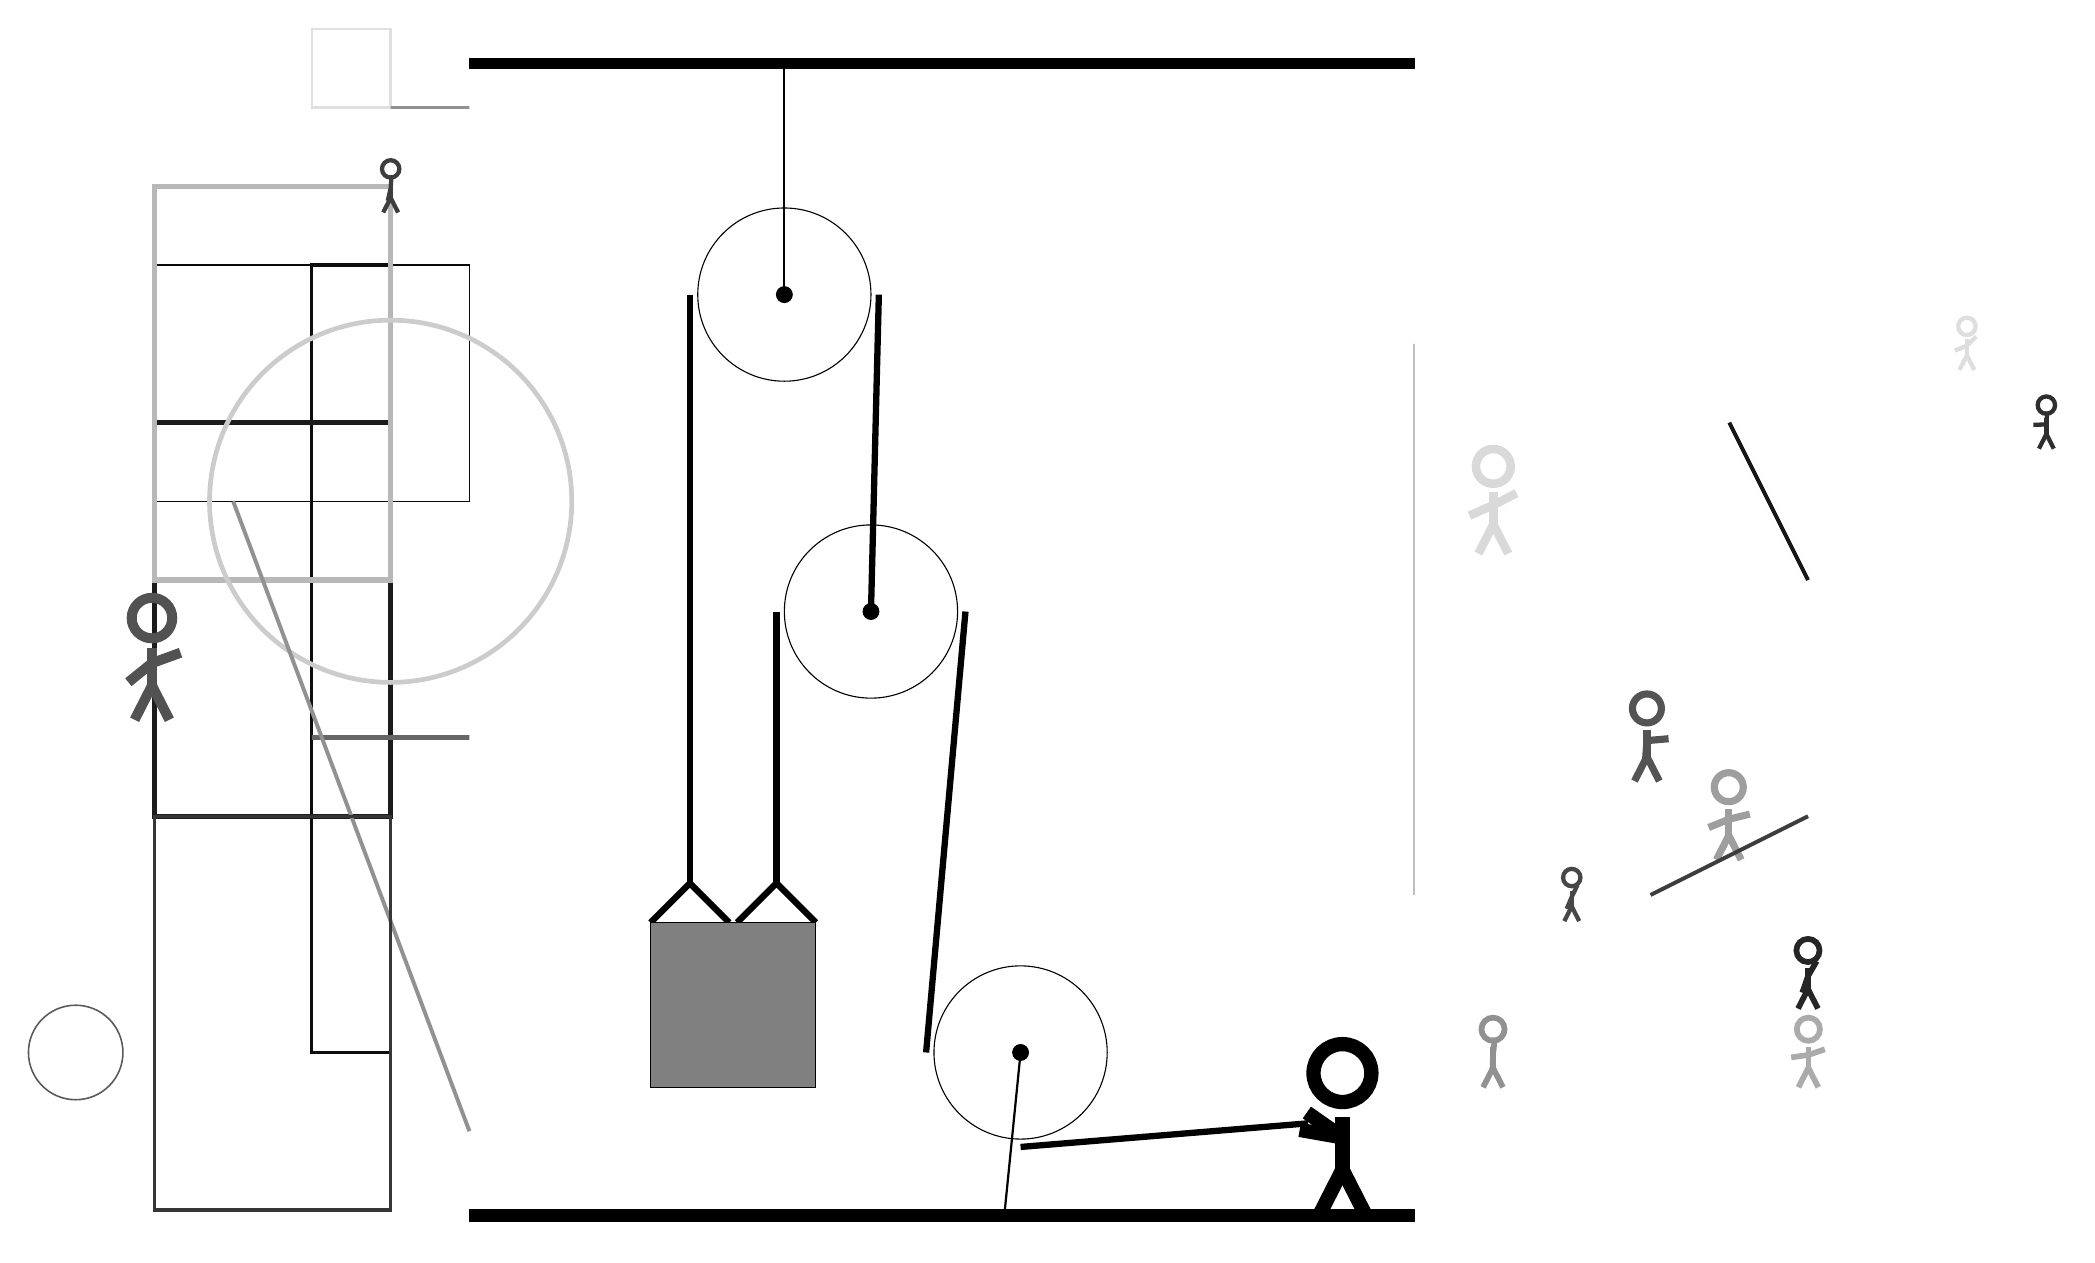
\begin{tikzpicture}
			%%%%% START %%%%%
			
			\draw[fill=black] (-2, 11.5) rectangle (10, 11.625);
			
			\draw (2, 8.625) circle (1.1);
			\draw[fill=black] (2, 8.625) circle (0.1);
			\draw[thick] (2, 8.625) -- (2, 11.5);
			
			\draw (3.1, 4.6) circle (1.1);
			\draw[fill=black] (3.1, 4.6) circle (0.1);
			
			\draw (5, -1) circle (1.1);
			\draw[fill=black] (5, -1) circle (0.1);
			\draw[thick] (5, -1) -- (4.8, -3);
			
			\draw[line width = 0.8mm]  (0.3, 0.65) -- (0.8, 1.15) -- (1.3, 0.65);
			\draw[line width = 0.8mm]  (1.4, 0.65) -- (1.9, 1.15) -- (2.4, 0.65);
			\draw[fill=black!50] (0.3, 0.65) rectangle (2.4, -1.45);
			
			\draw[line width = 0.8mm] (0.8, 8.625) -- (0.8, 1.15);
			\centerarc[line width = 0.8mm](2, 8.625)(0:180:1.2000000000000002);
			\draw[line width = 0.8mm] (3.2, 8.625) -- (3.1, 4.6);
			\draw[line width = 0.8mm] (1.9, 4.6) -- (1.9, 1.15);
			\centerarc[line width = 0.8mm](3.1, 4.6)(0:180:1.2000000000000002);
			\draw[line width = 0.8mm] (4.3, 4.6) -- (3.8, -1);
			\centerarc[line width = 0.8mm](5, -1)(180:270:1.2000000000000002);
			\draw[line width = 0.8mm] (5, -2.2) -- (8.65, -1.9);
			
			\node at (9, -2) {\Strichmaxerl[10][-35][170]};
			
			\draw [line width=0.2mm, color=black!65](-7, -1) circle (0.6);
			
			\node[line width=0.5mm, color=black!82] at (18, 7) {\Strichmaxerl[3][2][86]};
			\draw[line width=0.5mm, color=black!91](15, 5) -- (14, 7);
			\node[line width=0.5mm, color=black!33] at (15, -1) {\Strichmaxerl[4][8][19]};
			
			\draw[line width=0.5mm, color=black!47] (-4, 5) rectangle (-5, 5);
			\node[line width=0.5mm, color=black!13] at (17, 8) {\Strichmaxerl[3][22][45]};
			\draw[line width=0.2mm, color=black!97] (-2, 6) rectangle (-6, 9);
			\draw[line width=0.4mm, color=black!95] (-4, -1) rectangle (-3, 9);
			\draw[line width=0.6mm, color=black!89] (-3, 2) rectangle (-6, 7);
			\draw[line width=0.5mm, color=black!10](10, 3) -- (10, 3);
			\node[line width=0.5mm, color=black!85] at (15, 0) {\Strichmaxerl[4][71][60]};
			
			\draw[line width=0.7mm, color=black!28] (-3, 10) rectangle (-6, 5);
			\draw [line width=0.6mm, color=black!20](-3, 6) circle (2.3);
			
			\draw[line width=0.7mm, color=black!60] (-2, 3) rectangle (-4, 3);
			\node[line width=0.6mm, color=black!38] at (14, 2) {\Strichmaxerl[5][22][14]};
			\node[line width=0.2mm, color=black!68] at (-6, 4) {\Strichmaxerl[7][39][20]};
			
			\draw[line width=0.5mm, color=black!43](-5, 6) -- (-2, -2);
			\draw[line width=0.3mm, color=black!12] (-3, 11) rectangle (-4, 12);
			\node[line width=0.5mm, color=black!76] at (-3, 10) {\Strichmaxerl[3][77][86]};
			\node[line width=0.5mm, color=black!43] at (11, -1) {\Strichmaxerl[4][88][84]};
			\draw[line width=0.4mm, color=black!79] (-3, -3) rectangle (-6, 2);
			\draw[line width=0.3mm, color=black!25] (10, 8) rectangle (10, 1);
			\node[line width=0.6mm, color=black!15] at (11, 6) {\Strichmaxerl[6][24][27]};
			\draw[line width=0.5mm, color=black!76](15, 2) -- (13, 1);
			\node[line width=0.5mm, color=black!67] at (13, 3) {\Strichmaxerl[5][86][5]};
			\node[line width=0.3mm, color=black!72] at (12, 1) {\Strichmaxerl[3][67][64]};
			
			\draw[line width=0.3mm, color=black!43] (-2, 11) rectangle (-3, 11);
			
			\draw[fill=black] (-2, -3) rectangle (10, -3.15);
			
			%%%%% END %%%%%
		\end{tikzpicture}
	\end{figure}	
\end{document}